\documentclass[10pt,a4paper]{scrartcl}

% ── Page layout ───────────────────────────────────────────────────────────────
\usepackage[a4paper, top=15mm, bottom=15mm, left=18mm, right=18mm]{geometry}
\pagestyle{empty}

% ── Typography ────────────────────────────────────────────────────────────────
\usepackage{lmodern}
\usepackage[T1]{fontenc}
\usepackage[utf8]{inputenc}
\usepackage{microtype}

% ── Packages ──────────────────────────────────────────────────────────────────
\usepackage{graphicx}
\usepackage{booktabs}
\usepackage{xcolor}
\usepackage{colortbl}
\usepackage{enumitem}
\usepackage{caption}
\usepackage{float}
\usepackage{multicol}
\usepackage[hidelinks]{hyperref}

% ── Spacing tweaks ────────────────────────────────────────────────────────────
\usepackage[small,compact]{titlesec}
\titleformat{\section}{\large\bfseries\color{headerblue}}{}{0pt}{}[\vspace{1pt}\color{rulecolor}\hrule]
\titlespacing{\section}{0pt}{8pt}{4pt}
\titleformat{\subsection}{\normalsize\bfseries\color{headerblue}}{}{0pt}{}
\titlespacing{\subsection}{0pt}{6pt}{2pt}

\setlength{\floatsep}{4pt}
\setlength{\textfloatsep}{6pt}
\setlength{\intextsep}{4pt}
\setlength{\abovecaptionskip}{4pt}
\setlength{\belowcaptionskip}{2pt}

\setlist{nosep, leftmargin=1.2em}
\setlength{\parindent}{0pt}
\setlength{\parskip}{3pt}

\captionsetup{font=small, labelfont=bf, skip=4pt}

% ── Colors ────────────────────────────────────────────────────────────────────
\definecolor{headerblue}{HTML}{1B2A4A}
\definecolor{rulecolor}{HTML}{3366AA}
\definecolor{oomgreen}{HTML}{C8E6C9}
\definecolor{oomyellow}{HTML}{FFF9C4}
\definecolor{oomorange}{HTML}{FFCCBC}
\definecolor{oomred}{HTML}{EF9A9A}
\definecolor{goodrow}{HTML}{E8F5E9}
\definecolor{badrow}{HTML}{FFEBEE}
\definecolor{footergray}{HTML}{888888}

% ═════════════════════════════════════════════════════════════════════════════
\begin{document}

% ── Title block ───────────────────────────────────────────────────────────────
\begin{center}
  {\Large\bfseries\color{headerblue} RocksDB on Memory-Constrained Edge Devices}\\[5pt]
  {\normalsize Preliminary Benchmark Results\enspace---\enspace 4~March~2026}\\[2pt]
  {\small\color{footergray} Bachelor Thesis: Out-of-Core State Management for NebulaStream}
\end{center}
\vspace{-1mm}

% ── Background ────────────────────────────────────────────────────────────────
\section{Background}

\textbf{The problem.}\enspace
NebulaStream is a stream processing engine designed for IoT and smart city
deployments. Sensors (traffic cameras, air-quality monitors, smart meters)
produce continuous data streams that must be processed on cheap edge hardware
--- devices like the Raspberry Pi Zero~W with only 512\,MB of total RAM
($\sim$256\,MB available to applications). Stream operators such as windowed
aggregations and joins accumulate \emph{state} (e.g.\ partial sums, buffered
tuples) that can exceed available memory. An \emph{out-of-core} storage engine
is needed to spill this state to disk gracefully instead of crashing.

\textbf{Why RocksDB?}\enspace
RocksDB is an embedded key-value store built on the \emph{Log-Structured Merge
Tree} (LSM-tree) architecture. Incoming writes go into an in-memory buffer
called a \emph{memtable} (sized by \texttt{write\_buffer\_size}). When the
memtable is full it is \emph{flushed} to disk as a sorted file. Over time,
background \emph{compaction} merges these files to keep read performance
manageable. A \emph{block cache} (sized by \texttt{cache\_size}) keeps
frequently-read disk blocks in RAM. Because RocksDB is embeddable (no separate
server process) and widely used in production systems (MySQL/MyRocks, CockroachDB,
Kafka Streams), it is a natural candidate for NebulaStream's state backend.

\textbf{What we measure.}\enspace
This benchmark asks: \emph{can RocksDB operate reliably under the severe memory
constraints of an edge device, and which tuning knobs matter most?}

% ── How to read ───────────────────────────────────────────────────────────────
\section{How to Read This Report}

The following metrics appear throughout the results and findings:

\begin{description}[style=nextline, nosep, leftmargin=1.2em, font=\bfseries]
  \item[ops/sec (throughput)]
    Operations completed per second. Higher is better. One ``operation'' is one
    key-value read or write. This is the primary performance indicator.
  \item[p99 latency ($\mu$s)]
    The response time below which 99\,\% of operations complete, measured in
    microseconds. It captures worst-case user-visible delay. Lower is better.
  \item[Write amplification (W.Amp)]
    The ratio of bytes physically written to disk versus bytes the application
    intended to write. A value of 4$\times$ means each byte of user data causes
    4~bytes of disk I/O (due to repeated compaction). High write amplification
    wears out SD cards on edge devices and competes for I/O bandwidth.
  \item[Stall\,\% (write stalls)]
    The fraction of wall-clock time RocksDB spent \emph{blocking} new writes
    because its internal buffers or compaction pipeline were overloaded. During a
    stall, the stream processing pipeline cannot ingest new sensor data ---
    back-pressure propagates upstream and delays all operators.
  \item[Block cache hit rate]
    The fraction of read requests served from the in-memory cache rather than
    from disk. Higher hit rates reduce disk I/O and improve read latency.
  \item[OOM kill]
    When total memory usage exceeds the 256\,MB container limit, the Linux
    kernel's Out-Of-Memory killer terminates the process immediately. The run
    produces no results. This simulates a device crash in production.
  \item[write\_buffer\_size]
    Size of the in-memory write buffer (memtable). Larger buffers batch more
    writes before flushing to disk, reducing write amplification --- but consume
    more RAM and risk OOM kills.
  \item[cache\_size]
    Size of the block cache that keeps frequently-accessed disk data in RAM.
    Larger caches improve read performance but leave less memory for write
    buffers and the application itself.
  \item[Compression (none / snappy / lz4 / zstd)]
    Data can be compressed before writing to disk. Compression reduces disk I/O
    and storage footprint at the cost of CPU time. \texttt{snappy} and
    \texttt{lz4} are fast, lightweight codecs; \texttt{zstd} compresses more
    aggressively but uses more CPU.
\end{description}

% ── Experiment setup ──────────────────────────────────────────────────────────
\section{Experiment Setup}

We evaluate RocksDB as an embedded storage backend for stateful stream operators
on IoT-class edge devices. A Docker container enforces a hard 256\,MB memory
limit (swap disabled, single CPU) to simulate a Raspberry Pi Zero~W deployment.
The \texttt{readwhilewriting} workload models a stream processing scenario:
concurrent state lookups while sensor data is being ingested.

\smallskip
\begin{tabular}{@{}ll@{\qquad}ll@{}}
  \textbf{Dataset:}   & 2\,M keys $\times$ (16\,B key + 100\,B value) $\approx$ 230\,MB on disk &
  \textbf{Memory:}    & 256\,MB (cgroup-enforced, no swap) \\
  \textbf{Sweep:}     & 4 compression $\times$ 5 write\_buffer $\times$ 5 cache\_size = 100 runs &
  \textbf{Outcome:}   & 58 succeeded, 42 OOM-killed \\
\end{tabular}

% ── Figure 1: Throughput ──────────────────────────────────────────────────────
\section{Results}

\begin{figure}[H]
  \centering
  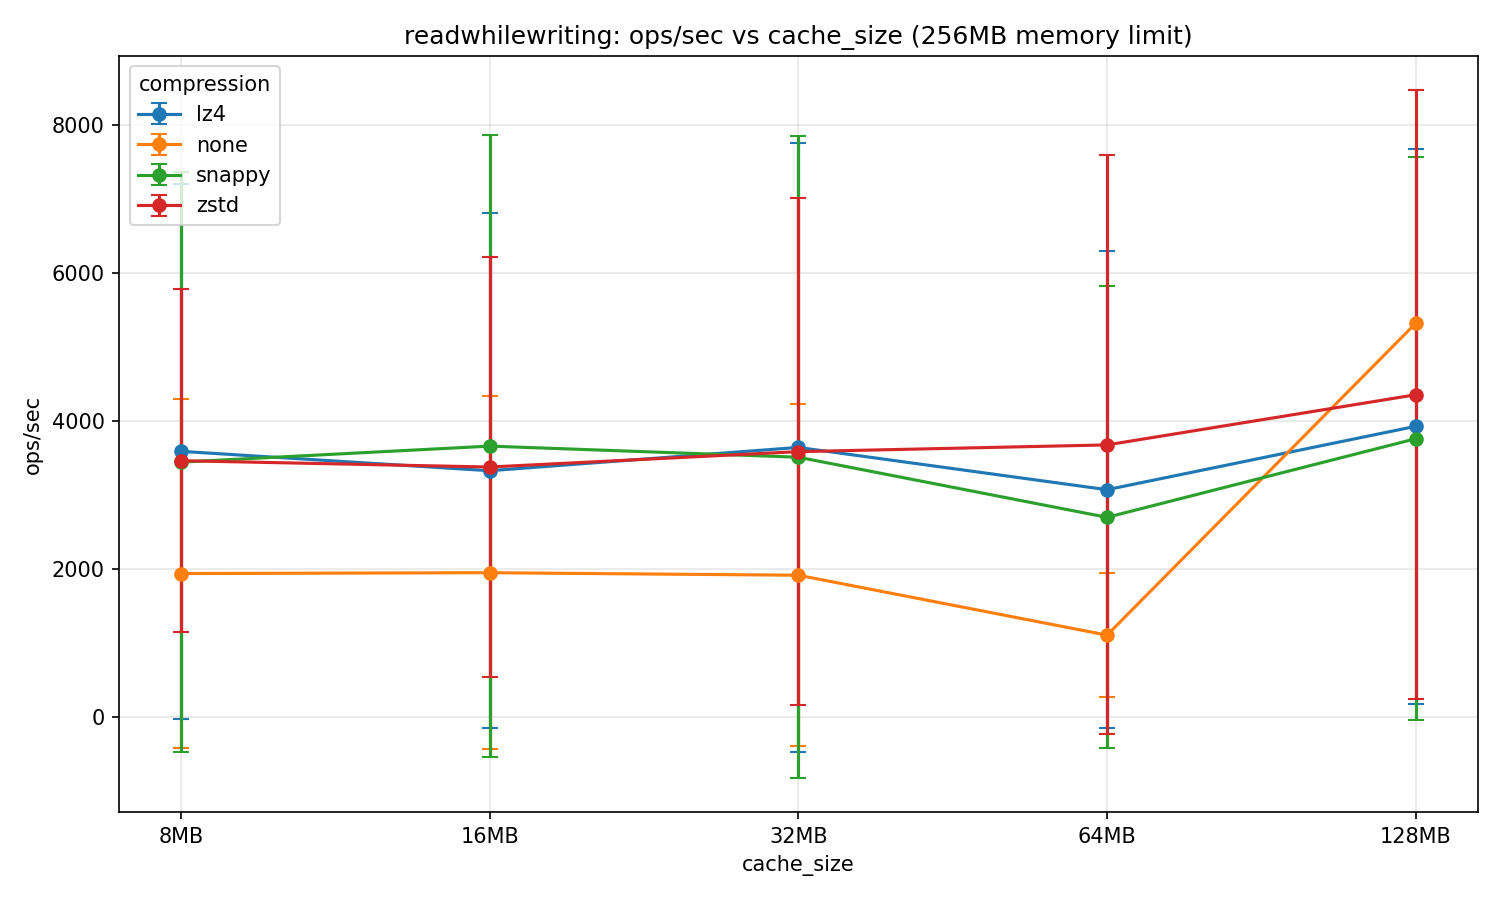
\includegraphics[width=0.92\textwidth]{parsed/plot_readwhilewriting_ops_vs_cache_size.png}
  \caption{Throughput (ops/sec) vs.\ block cache size, grouped by compression algorithm.
           Error bars show standard deviation across \texttt{write\_buffer\_size} values.
           Compressed codecs (lz4, snappy, zstd) consistently outperform uncompressed
           storage by 1.5--2$\times$.}
\end{figure}

% ── Figure 2: Write stalls ───────────────────────────────────────────────────
\begin{figure}[H]
  \centering
  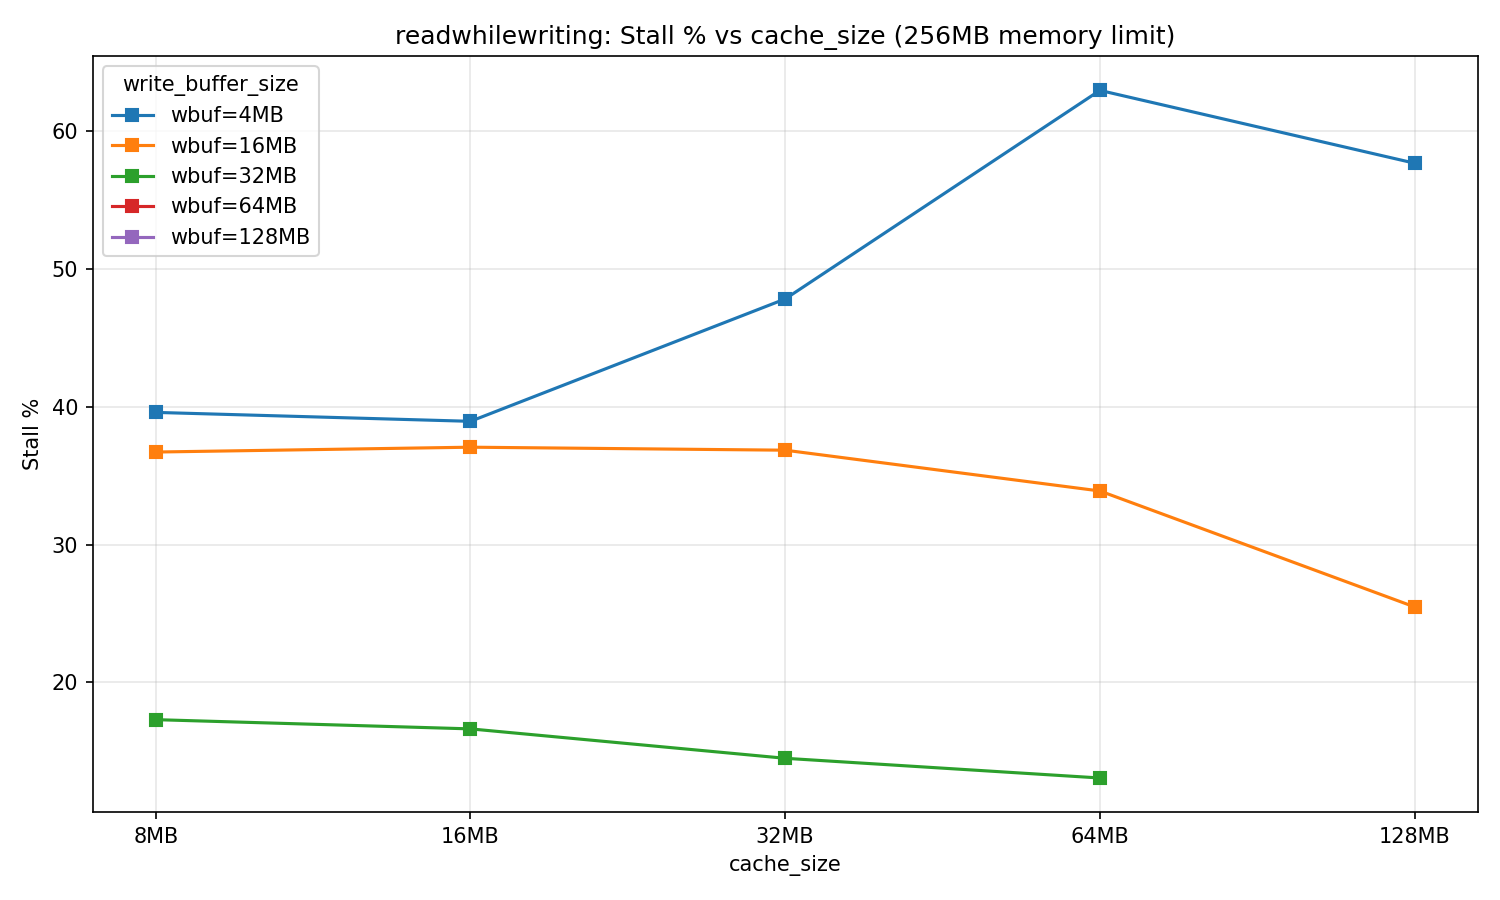
\includegraphics[width=0.92\textwidth]{parsed/plot_readwhilewriting_stalls_vs_cache_size.png}
  \caption{Write stall percentage vs.\ block cache size, grouped by
           \texttt{write\_buffer\_size}. Smaller write buffers (4\,MB) flush frequently,
           causing high stall rates (40--63\,\%) but completing each flush quickly.
           Larger buffers (32\,MB) stall less (15\,\%) but individual flushes are
           more expensive under memory pressure.}
\end{figure}

% ── Figure 3: Write amplification ────────────────────────────────────────────
\begin{figure}[H]
  \centering
  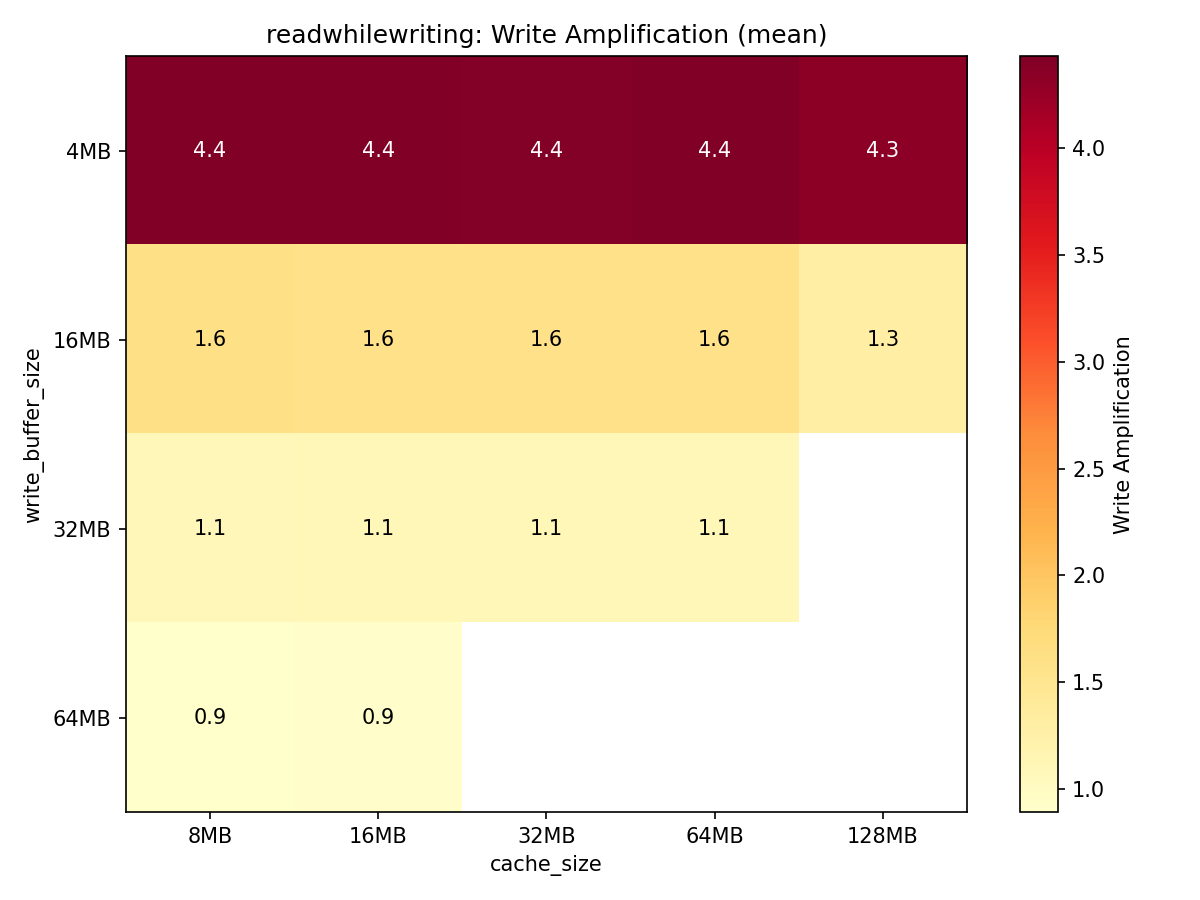
\includegraphics[width=0.72\textwidth]{parsed/plot_readwhilewriting_write_amp_heatmap.png}
  \caption{Write amplification heatmap (\texttt{write\_buffer\_size} $\times$
           \texttt{cache\_size}). A 4\,MB write buffer produces 4.4$\times$ write
           amplification due to frequent compaction, while 64\,MB achieves near-optimal
           0.9$\times$ --- but at the cost of OOM kills in most configurations.}
\end{figure}

\newpage

% ── Key findings ──────────────────────────────────────────────────────────────
\section{Key Findings}

\subsection{1\enspace---\enspace OOM Kill Boundary}

The matrix below shows the fraction of runs killed per configuration.
\texttt{write\_buffer\_size} is the dominant factor: $\geq$\,64\,MB is
essentially unusable on a 256\,MB device regardless of cache allocation.

\medskip
{\centering
\begin{tabular}{lcccccc}
  \toprule
  & \multicolumn{5}{c}{\textbf{cache\_size}} \\
  \cmidrule(lr){2-6}
  \textbf{write\_buffer\_size} & \textbf{8\,MB} & \textbf{16\,MB} & \textbf{32\,MB} & \textbf{64\,MB} & \textbf{128\,MB} \\
  \midrule
  4\,MB   & \cellcolor{oomgreen}0/4  & \cellcolor{oomgreen}0/4  & \cellcolor{oomgreen}0/4  & \cellcolor{oomgreen}0/4  & \cellcolor{oomgreen}0/4 \\
  16\,MB  & \cellcolor{oomgreen}0/4  & \cellcolor{oomgreen}0/4  & \cellcolor{oomgreen}0/4  & \cellcolor{oomgreen}0/4  & \cellcolor{oomyellow}1/4 \\
  32\,MB  & \cellcolor{oomgreen}0/4  & \cellcolor{oomgreen}0/4  & \cellcolor{oomgreen}0/4  & \cellcolor{oomgreen}0/4  & \cellcolor{oomred}4/4 \\
  64\,MB  & \cellcolor{oomyellow}2/4 & \cellcolor{oomorange}3/4 & \cellcolor{oomred}4/4    & \cellcolor{oomred}4/4    & \cellcolor{oomred}4/4 \\
  128\,MB & \cellcolor{oomred}4/4    & \cellcolor{oomred}4/4    & \cellcolor{oomred}4/4    & \cellcolor{oomred}4/4    & \cellcolor{oomred}4/4 \\
  \bottomrule
\end{tabular}
\par}

\medskip
\textbf{Safe operating zone:} write\_buffer $\leq$\,32\,MB combined with cache $\leq$\,64\,MB.

\subsection{2\enspace---\enspace Compression Is Critical}

\begin{tabular}{lrrrr}
  \toprule
  \textbf{Compression} & \textbf{ops/sec} & \textbf{p99 ($\mu$s)} & \textbf{Write Amp.} & \textbf{Stall\,\%} \\
  \midrule
  \rowcolor{goodrow} \textbf{zstd}   & 3{,}627 & 3{,}187  & 1.79 & 31.6 \\
  \rowcolor{goodrow} lz4             & 3{,}474 & 4{,}823  & 1.91 & 28.6 \\
  snappy                             & 3{,}384 & 6{,}636  & 2.07 & 27.6 \\
  \rowcolor{badrow}  none            & 1{,}998 & 11{,}917 & 3.93 & 50.8 \\
  \bottomrule
\end{tabular}

\smallskip
Running without compression is catastrophic under memory pressure: throughput
drops 1.8$\times$, write amplification doubles to 3.9$\times$, and the engine
spends over 50\,\% of its time stalled. \textbf{zstd} delivers the best
throughput and lowest tail latency despite its higher CPU cost on a single core.

\subsection{3\enspace---\enspace 17$\times$ Performance Cliff}

\begin{tabular}{lrr}
  \toprule
  \textbf{Configuration} & \textbf{ops/sec} & \textbf{p99 ($\mu$s)} \\
  \midrule
  \rowcolor{goodrow} wbuf=4\,MB, lz4, cache=8\,MB    & \textbf{8{,}900} & 354 \\
  \rowcolor{goodrow} wbuf=4\,MB, snappy, cache=32\,MB & 8{,}510          & 670 \\
  \rowcolor{badrow}  wbuf=16\,MB, none, cache=16\,MB  & \textbf{518}     & 19{,}761 \\
  \rowcolor{badrow}  wbuf=16\,MB, none, cache=32\,MB  & 518              & 19{,}497 \\
  \bottomrule
\end{tabular}

\smallskip
Within the same 256\,MB budget, configuration choices alone produce a
\textbf{17$\times$ throughput difference}. This demonstrates that tuning knob
selection dominates hardware constraints for RocksDB on edge devices.

\subsection{4\enspace---\enspace Write Stalls Back-Pressure the Pipeline}

\begin{itemize}
  \item Mean stall time: \textbf{34.3\,\%}, maximum: \textbf{71.8\,\%}. 14 of 58 successful runs spent more than half their time stalled.
  \item Paradox: a 4\,MB write buffer has the highest stall percentage ($\sim$40--63\,\%) but also the highest throughput --- frequent small flushes complete faster than infrequent large ones under memory pressure.
  \item \textbf{NebulaStream implication:} RocksDB write stalls propagate as back-pressure through the entire stream processing pipeline, blocking upstream operators.
\end{itemize}

\subsection{5\enspace---\enspace Block Cache Hit Rate}

\begin{tabular}{lccccc}
  \toprule
  \textbf{cache\_size} & \textbf{8\,MB} & \textbf{16\,MB} & \textbf{32\,MB} & \textbf{64\,MB} & \textbf{128\,MB} \\
  \midrule
  Hit rate             & 4.5\%          & 9.3\%           & 18.8\%          & 32.9\%          & 64.1\% \\
  \bottomrule
\end{tabular}

\smallskip
The hit rate scales approximately linearly with cache size --- no sudden cliff.
A 32\,MB cache (12.5\,\% of device RAM) achieves 18.8\,\% hit rate, offering
a reasonable trade-off between memory reserved for stream operators and storage
performance.

% ── Next steps ────────────────────────────────────────────────────────────────
\section{Next Steps}

\begin{enumerate}
  \item Run the full parameter sweep (900 combinations) including
        \texttt{level0\_slowdown\_writes\_trigger} and
        \texttt{min\_level\_to\_compress} variations.
  \item Add the \texttt{fillrandom} workload to capture pure write (sensor ingestion) performance.
  \item Evaluate with NebulaStream-realistic key/value sizes to validate external applicability.
\end{enumerate}

\vfill
\noindent\color{footergray}\rule{\textwidth}{0.3pt}\\[2pt]
{\footnotesize\color{footergray}
  Microbenchmark-BA\enspace$\bullet$\enspace
  100 overnight runs\enspace$\bullet$\enspace
  Docker \texttt{--memory=256m --memory-swap=256m --cpus=1}\enspace$\bullet$\enspace
  RocksDB \texttt{db\_bench}\enspace$\bullet$\enspace
  2\,M keys, 16\,B key + 100\,B value}

\end{document}
